\section{Monte Carlo Study}

\subsection{Convergence}

We calculate statistical models with bayesian methods by typically drawing random samples from the underlying distribution. As shown in the previous chapter we use Markov chain Monte Carlo methods like the Metropolis hastings algorithm, because they converge to the equilibrium of the model. Once we have achieved convergence the following draws will be drawn from the underlying distribution. \\
Since bayesian estimation methods are computationally intensive, there is a great demand for methods that reliably determine convergence.\\
As a first step, the first half (or quarter) of draws should be discarded to mitigate the the influence of the initial parameters and allow the algorithm time to converge. In the next step we test wether the algorithm is converged and extend the burn-in period if not.
Since parameter draws with a higher posterior value are accepted more frequentuently the chain flucuates around the posterior mode once it has converged. Therefore a graphical analysis of the draws is a frequently used technique to monitor convergence..\\
Also, parts of the chain can be compared with each other using statistical methods. The idea is that if both are from the same distribution, they must be sufficiently similar.For example, the Gekwek convergence criterion compares the parameter mean of the first 10\% and 50\% of the draws while taking the autocorrelation of draws into account \cite{geweke1992}.\\
However, \cite{brooks1998} argue that it is not possible to determine convergence with a single chain.As with many other iterative optimizations the optimizer can get stuck in a region with a low density for a long time.Therefor, one should start with several highly dispersed starting values to detect false convergence with a higher probability. In a well-known paper \cite{gelman1992} instead proposes to compare the variance of several parallel chains.
We follow their approach and calculate the brook and gelman convergence criteria to capture convergence in our simulation study.\\
To do this, we start several chains M$\geq$2 with N draws (after the burn-in period). 
For every paramter of our model, we calculate the chain variance $s_m^2$ as $\frac{1}{N-1}\sum_{n=1}^{N} (\theta_m^{(n)}-\overline{\theta}_m )^2$ using $\overline{\theta}_m=\frac{1}{N} \sum_{n=1}^{N} \theta_m^{(n)}$.\\
We derive the average within-chain-variance W by averaging over all M chains.\\
$$W=\frac{1}{M} \sum_{m=1}^{M} s_m^2 $$ 
And calculate the between sequence variance B/N as:
$$B/N=\frac{1}{M-1} \sum_{m=1}^{M} (\overline{\theta}_m-\overline{\theta} )^2 $$
using the average draw of all chains $\overline{\theta}=\frac{1}{M} \sum_{m=1}^{M} \theta_m$.
Brooks and Gelman derive an estmate of the total variance as a weighted sum of with-in chain variance and between chain variance.
$$\widehat{var}^+ (\theta \mid y)=\frac{N-1}{N}W+\frac{1}{N}B$$
This estimate will be unbiased when we reached convergence and will overestimate the variance when we start with widely distributed inital values.
If we take our sampling uncertainty about our posterior mean $\overline{\theta} $ into account we derive the posterior Variance estimate $\widehat{V}$ as $\widehat{var}^+ (\theta \mid y) +\frac{B}{MN}$ \cite{brooks1998}
The second part of the equation is often neglected as N is large enough in most circumstances (for example Stan uses the simplified version).
Finally, the potential scale reduction statistic is defined by the equation:
$$\widehat{R}=\sqrt{\frac{\widehat{V}}{W}}$$
If the algorithm converged, then the whole variance follows from the underlying distribution. The within-chain variance is large compared to the between-chain variance and $ \widehat{R}$ is close to 1.\\
$\widehat{R}$ is much bigger if the estimate of the total variance is poor. Or if there are big differences between the different chains, because they did not converge to the same value.  In both cases, we should increase the number of iterations. In general, a scale reduction factor below 1.1 strongly suggests overall convergence, while a scale reduction factor below 1.2 weakly suggests.\cite{brooks1998}



\subsection{Stan Configurations}
We use the open-source package Stan for the calculation of  Bayesian hierarchical models. Stan is an  C\texttt{++} package with its programming language for coding probability models.  Bayesian models can be fit with bayesian and maximum likelihood methods. We accessed Stan via the interface Pystan in the programming language Python. Because Stan compiles our model into C\texttt{++} code, we can realize fast run times using a standard laptop.\\
Stan uses the Nuts-Sampling algorithm based on the Hamilton Monte Carlo (HMC) with the advantage  over other Markov Chain Monte Carlo methods that it produces distant candidate draws, hereby incresasing effective sample size and convergence of the algorithm.
On the other hand, the efficiency of HMC is highly sensitive to tuning parameters leapfrog stepsize $\epsilon$ and number of leapfrog steps, L. \cite{neal2011}. % write sentence about Hamiton monte Carlo leapfrog and steps form neal
The invention of the no-u turn sampler has opened the use of the HMC to many other areas by automatically settting optimal parameter values for leapfrog stepsize and leapfrog steps.\cite{hoffman2014}  \\
%Stan uses the hamilton monte carlo modified around the no-uturn sampler and we use it exclusively in our monte carlo study. The first part of burn-in perior is used to tune the parameters of the model.
%For every (current) trajectory Stan measures how 
%Stan measures how the (current) trajectory would lead the MCMC to new areas. If this trajectory would lead it far from the posterior mean, it will report a high divergence value, and we risk wandering around areas with a low posterior value for a long time. By setting a higher target acceptance, we (indirectly) decrease the stepsize, because variables with higher posterior values will be accepted more often. Consequently, we limit the sampled region of the posterior.
%We might want to use a higher acceptance rate of $\delta$ if we have to happen a high convergence in our draws. For every draw, 
%Depending on the convergence results of our Monte Carlo runs (and friendly recommendations of Stan) we change the (target) acceptance rate $\delta$.\\
%By setting $\delta$, we can change the (expected) probability that a draw with a smaller posterior value lowe, then the value of the current draw is kept. The default value of the target acceptance rate is 0.8, which happens to be around the optimal value under some normality assumptions. Roberts, Gelman, and Gilks (1997). \cite{roberts1997b}
%In Stan this target acceptance rate influences the stepsize of the Hamilton Monte Carlo algorithm. A higher stepsize increase the range of possible candidate draws around the current draw $\theta_i$. Therefore if we have a high stepsize (and we are currently around the posterior mean), many draws with a low posterior value will be proposed and subsequently rejected. If the step size is too small, we will accept many draws, but most of them will be in the small distance to the posterior mean. Therefore we will need a long time to discover the full posterior distribution. \cite{stan2018}

We can further increase the efficency of the Markov Chain monte Carlo algorithm by starting with initial values close the posterior mean. Because this value is unknown ex ante a common strategy is to find the posterior mean first with a numerical optimizer (e.g., Stan uses the quasi-newton algorithms LBFGS as a default). Then we sample intial values for our M chains from a fat tailed distribution like the t-distribution.\cite{brooks1998}
As seen in figure \ref{fig:convergence}, Hamilton monte carlo encountered no problems to finding the posterior mode of our simple models. Therefor we use the default option of stan - Initial values are drawn from the UNI[-2,2]. If parameters are constrained, they are transformed into the unconstrained space before. For example, intial values of the standard deviation are drawn from the intervall $[e^{-2},e^2]$.   

\begin{figure}[h!]
  \centering
  \begin{subfigure}{0.3\linewidth}
    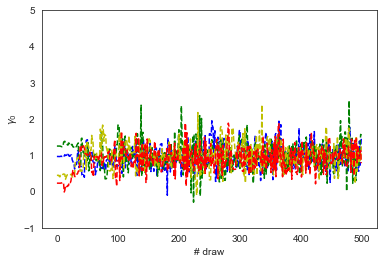
\includegraphics[width=\linewidth]{graphics/convergence}
    \caption{Paramter draws of 4 chains.}
  \end{subfigure}
  \caption{First 500 parameter draws of $\gamma_0$ with our second DGP.}
  \label{fig:convergence}
\end{figure}

\subsection{Monte Carlo Preparations}
% introduce model
In our monte carlo study we ask ourselves how the calculation of bayesian hierarchical models reacts to different prior distributions on our hyperparameters.
We analyze the performance in respect to the random slope model with group characteristics.

\begin{align}
  y_i &= \alpha+ x_i^\prime \beta_{j[i]} + \epsilon_i \,,\\
  \beta_{j[i]} &= \gamma_0 + u_j^\prime \gamma + \eta_j \,,
\end{align}

Varying slope models are widely used in political science, educational research and psychology. For example, \cite{snijders2012} researchers can use such a model to test the effects of social status($x_i$) on the left-right positioning ($y_i$) of individuals. The impact of social status on political affiliation $\beta_{j[i]}$ are allowed to be different for individuals of different countries J. They depend on the level of inequality in this country ($u_j$)  and random effects $\eta$.\\
If $u_j$ is demeaned, we can interpreted $\gamma_0$  as the constant effect of inidividual characteristic, while $\gamma_1$ indicates how group-characteristics shape the effects of individual characteristics.\\
In our simulation study we analyze the performance of bayesian models by determining both parameters. We fix the group characteriscs $u_j$ and individual characteristcs $x_i$, but draw new realizations of  $\eta$, and $\epsilon$ in every simulation run.\\

We tested two different data generating processes in our analysis: \\

1) we used non-centered characteristics $u_j$ and $x_i$ as\\

$x_i \sim N(5,0.3)$ , $\epsilon \sim N(0,\sigma_y) $ , $U_j \sim N(5,0.3)$ , $\eta \sim N(0,1) $ , $\eta \sim N(0,\sigma_b)$\\
and fixed parameters $\alpha=1$, $\gamma_0=1$ , $\gamma_1=1$ , $\sigma_b=\sigma_y=1$\\

2) we used centered characteristics and included more variation in our data: \\ 

$x_i \sim N(0,3)$ ,  $\epsilon \sim N(0,\sigma_y) $ , $U_j \sim N(0,3)$ , $\eta \sim N(0,1) $ , $\eta \sim N(0,\sigma_b)$\\
and fixed parameters $\alpha=1$, $\gamma_0=1$ , $\gamma_1=1$ , $\sigma_b=\sigma_y=1$ \\

% choosing the right prior
The selection of a meaningful prior distribution is the best known feature of bayesian statistics and a frequent source of criticism. In some situations we can incorporate external knowledge for determining prior distributions. For example, many macroeconomic studies estimate the discount factor beta  between 0.93 and 1 with the average around 0.99 for most countries.  \cite{rumler2007}
In other situations the information situation is unclear. While it is desired that our prior distribution will have direct conseqences on our estimates, it is not the desirable that the prior completely dominates the new information from the data ("let the data speak").\\
An extra difficulty comes from the fact that the strength of a prior can only be determined in the context of likelihood. It is therefore a common strategy to select prior distributions according to the data basis. \cite{gelman2017prior}. 
Often different prior designs are tested and selected based on their comparability to the data. \cite{leeper2017clearing}.
If the size of the effect is unknown in advance it also makes sense to normalize the input data. For example, the impact of wealth on risk aversion will change depending on the currency unit in which wealth is calculated. It was found that scaling of the input data also influences the efficiency of the algorithms.\cite{gelman2008weakly} \\
In our monte carlo study we test the effect of informative, weakly informative and uninformative prior distribuitons on our bayesian estimations.
The idea is to start with an informative prior distribution around the true mean of our parameters $\gamma_0=\gamma1=1$. Then we move the distribution of one unit in the wrong direction - so make it wrong and informative.
Next, we turn our prior distribution into a weakly informative one by increasing the standard distribution of priors from 1 to 3.
We also try a less shifted prior distribution and a uniform prior distribution. See Table \ref{tab:prior_table} for an overview of the prior distributions we have chosen.
In all our simulations we use a Half-Cauchy (0.5) prior for the standard deviations of the innovations. With an median of 5 it is very uninformative and will have a negligible influence on the results.
By default we calculate our models with 10 groups and 200 individuals per group, but we also look at the results of reducing the size and number of groups.All the simulations that do not converge are sorted out in the analysis. However, we require a total of 300 simulations for each model. Our standard stan parametrization can be found in the appendix. \ref{tab:default_1} \ref{tab:default_2}


\begin{table}[!ht]
\begin{center}
\begin{tabular}{l l l l l l}
Prior specification & Short-Name for Model & $\gamma_0$ & $\gamma_1$ & $\sigma_y$,$\sigma_\beta$\\
\hline
True, strong priors &  Truel & $N(1,1)$ & $N(1,1)$ & $C^+(0, 5)$\\
Wrong, strong priors & Wrong  &$N(2,1)$ & $N(2,1)$ & $C^+(0, 5)$\\
Wrong, weak priors &  Weakwrong  & $N(2,3)$ &$ N(2,3)$ & $C^+(0, 5)$\\
Slightly wrong, weak priors &  Weakslighltywrong & $N(1.2,3)$ &$ N(1.2,3)$ & $C^+(0, 5)$\\
Uniform prior & Uniform &$UNI[-\infty,\infty]$ & $UNI[-\infty,\infty]$ & $C^+(0, 5)$\\
\end{tabular}
\end{center}
\caption{The prior distributions of our hyperparameters $\gamma_0, \gamma_1, \sigma_\beta and  \sigma_y$}
\label{tab:prior_table}
\end{table}


\subsection{Monte Carlo Results}

In our Monte Carlo study we use the posterior mean as the point estimate models of our model parameters. Practioners also use the mode or median of the posterior. Because posterior distributions are not symmetric by nature the estimates will be different. 
However, the results were similar when we tried the median instead of the mean.\ref{tab:median}.
We assess the performance of bayesian method using four different criteria.
First, we calculate the average posterior mean of all of our sample runs. We use this metric to identify bias in our estimations. 
Second, we test calculate [$5\text{\%}$, $95\text{\%}$] intervalls posterior means in our 300 runs, to check how stable the results are for changes in input data.
Third, we calculate average [$5\text{\%}$, $95\text{\%}$] posterior intervalls. This metric gives us an estimate of the average uncertainty in the calculation of the parameters.
Forth we calculate [$2.5\text{\%}$, $97.5\text{\%}$] intervalls for our parameters in every simulation run. Then we count how many times the true parameter falls  inside of the intervall to test if our confidence intervalls are conservative or optimistic. Furthermore the [$2.5\text{\%}$, $97.5\text{\%}$] intervall - called credible set in the bayesian literature - are used by Researchers to determine the statistical significance of a parameter in Bayesian statistics. if the true value did not fall within this interval, we would have rejected it in our analysis. \cite{koop2003}.
As can be seen in table  \ref{tab:bias_first}  , our Bayesian Methods performed far worst for our first data-generating-process. We severly underestimate $\gamma_0$, while overestimating $\gamma_1$.
A reason for this is that the parameters of the group model are interdependent.A bias in one of the parameters worsens the calculation of all other parameters.  Therefore we expect a good fit for all parameters or none of them.  In the first DGP we can offset a underestimation of $\gamma_0$  by an increase in $\gamma_1$ if group characteristics are not centered around zero.\\
In accordance with the predictions of \cite{gelman2008weakly}, scaling of input variables had a big impact on the efficiency of our estimations as well. It took far longer to fit the model to our first data-generating process as Hamilton Monte Carlo showed slower convergence and more convergence. This means our first DGP shows anectdotal evidence that problems with fitting a model often arise because of wrong parametrization/modelling.\\

Consequently, we directed our further analysis to the second data generating process.% (See the appendix for results of the first model configuration).
First, we calculate the average posterior mean for $\gamma_0$,$\gamma_1$, $\sigma_b $ and $\sigma_y$ in all simulation runs.
As can be seen in table\ref{tab:bias_second} our estimate of $\sigma_y$ is very close to the true value regardless of prior selection or number of levels. This is not suprising since we work with large sample sizes in our model. 
The average mean of the intercept parameter $\gamma_0$ is close to true parameter as well. Although we observe that a wrong prior pulls the average estimate in its direction.
The slope parameter $\gamma_1$ was biased upwards in all of our simulation runs. The bias increases with a wrong prior. Interestingly, we decrease the bias by roughly 2/3 if we increase the standard deviation of our (wrong) prior distribution from 1 to 3. 
We overestimated the standard deviation $\sigma_b$ in all our configurations. This is not surprising since we only have 5-10 groups in our monte carlo and use a weakly informative prior distribution. Yet we can still observe that our bias in $\sigma_b$ increases when we have bias in other parameters as well. The only exception to this rule is the model with a uniform prior. Our estimates of the hyperparameters $\gamma_0$ and $\gamma_1$ are less biased, while the standard deviation $\sigma_b$ increase greatly.\\
 
Surprisingly the positive bias of $\gamma_0$ and $\gamma_1$ decreases when we decrease the number of individuals per group.\\
Alarmingly the average variance of $\sigma_b$ rises as well, which was connected with a worst fit in previous runs. That is why we take a further look at results of the model with a wrong prior, because we can observe the highest drop in bias here.
In Figure \ref{fig:various sample size} we plotted the density of the posterior mean of $\eta_1$ (the error realiziation of group 1) against the posterior mean of $\gamma_1$ for a wrong prior. While $\gamma_0$ is pulled towards 2 by the prior, we can see that their relationship is stable for 200 individuals per group.
However, once we use only 100 individuals per group many posterior means assemble around a new centre with a negative bias in $\gamma_1$ and a positive bias in $\eta_1$. Because our estimates have an positve bias for $\gamma_0$ in the old centre, the bias is partly cancelled out.
If we decrease the number of groups J, instead we increase the variance in our estimates, but do not create the unstable relation seen before.
See also \ref{fig:posterior_wrong_gamma0} and \ref{fig:posterior_wrong_gamma1} for the plottet posterior distributions. 

% continue from here
\begin{figure}[h!]
  \centering
  \begin{subfigure}[b]{0.3\linewidth}
    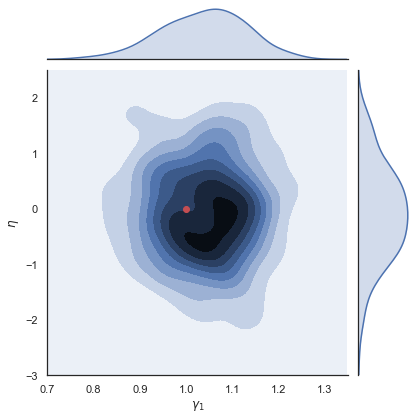
\includegraphics[width=\linewidth]{graphics/jointplot_gamma1eta_big}
    \caption{ N=200, J=10}
  \end{subfigure}
  \begin{subfigure}[b]{0.3\linewidth}
    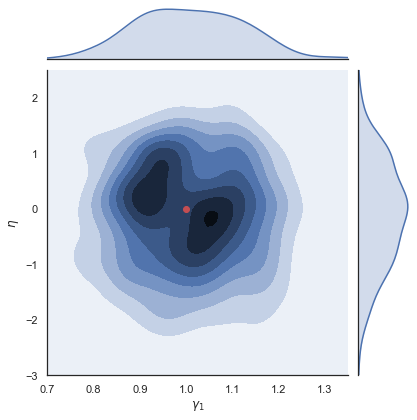
\includegraphics[width=\linewidth]{graphics/jointplot_gamma1eta_small}
    \caption{N=100, J=10}
  \end{subfigure}
  \begin{subfigure}[b]{0.3\linewidth}
    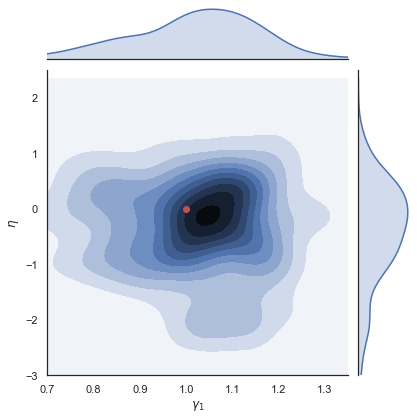
\includegraphics[width=\linewidth]{graphics/jointplot_gamma1eta_smallJ}
    \caption{ N=200, J=5}
  \end{subfigure}
  \caption{Joint-Posterior-Density of posterior mean estimates of $\gamma_1$ and $\eta$ of a model with a wrong prior.Red dot=Expected Value}
  \label{fig:various sample size}
\end{figure}



Next, we compare the posterior means of our simulation runs. As can be seen in figure \ref{fig: gamma0 and gamma1} , our estimate of $\gamma_0$ show higher variability then our estimates of $\gamma_1$. Since we work with a low number of groups J our estimates of the intecept will be heavily affected by our realizations $\eta$. Since our group characteristics are very informative in predicting the impact of individual characteristcs $\beta$,  $\gamma_1$  changes very little. 
On the other hand $\gamma_0$  reacts relatively strongly to different prior distributions, as the underlying data is varies widely.



In \ref{fig:gamma0_posterior}the next graph we compare the estimations of $\gamma_0$ in a model with a uniform and a wrong prior. We can observe that the wrong prior results in a higher bias in the estimates, while a uniform prior does introduce more variation in our model.
As can be seen in tabel \ref{tab:means} and figure \ref{fig:gamma0_posterior}a weakly informative prior can combine both strenghts by having a bias comparable to the bias of a uninformative prior while slightly reducing the variation in our model.
We can see that the wrong prior shifts the posterior distribution to the right and thereby increases the bias. A uniform prior does introduce more variability in our parameter estimates - the curvature of our posterior densities increases.
By using a wrong and weak prior we raise the bias of our estimate, but have a higher curvature of our posterior. The following graphs plots a densities of the posterior means against each other. The differences between both graphs are very small, but posterior density of the model with a weak prior has smaller tails, but a bigger bias. As seen in  the slightlywrong prior does dominate the uniform prior with a lower upper estimate and higher lower estimate.


\begin{figure}[h!]
  \centering
  \begin{subfigure}[b]{0.4\linewidth}
    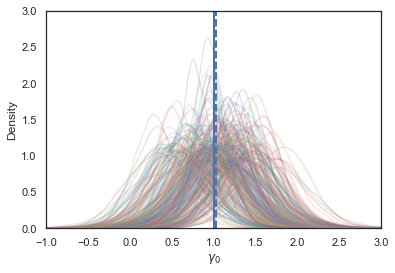
\includegraphics[width=\linewidth]{graphics/posterior_plot_gamma0}
    \caption{True Prior, N=100, J=10}
  \end{subfigure}
  \begin{subfigure}[b]{0.4\linewidth}
    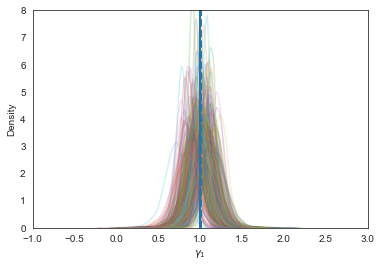
\includegraphics[width=\linewidth]{graphics/posterior_plot_gamma1}
    \caption{True Prior, N=200, J=10}
  \end{subfigure}
  \caption{Posterior densities  of $\gamma_0, \gamma_1$, Blue line: True Value, Dotted line: Average Estimate}
  \label{fig: gamma0 and gamma1}
\end{figure}

\begin{figure}[h!]
  \centering
  \begin{subfigure}[b]{0.4\linewidth}
    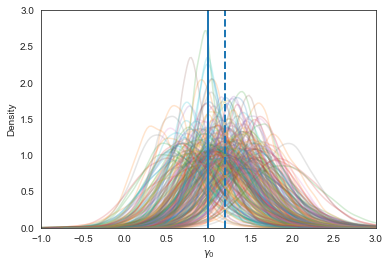
\includegraphics[width=\linewidth]{graphics/posterior_plot_gamma0_wrong}
    \caption{Wrong Prior, N=100, J=10}
  \end{subfigure}
  \begin{subfigure}[b]{0.4\linewidth}
    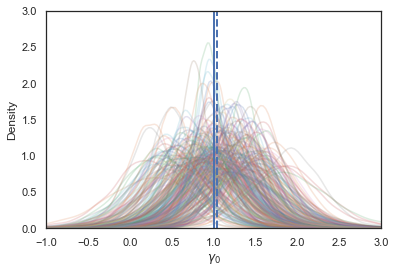
\includegraphics[width=\linewidth]{graphics/posterior_plot_gamma0_uni}
    \caption{Uni Prior, N=200, J=10}
  \end{subfigure}
  \caption{Posterior densities of $\gamma_0$, Blue line: True Value, Dotted line: Average Estimate}
  \label{fig:gamma0_posterior}
\end{figure}

\begin{figure}[h!]
  \centering
  \begin{subfigure}[b]{0.4\linewidth}
    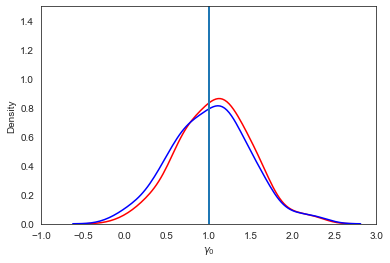
\includegraphics[width=\linewidth]{graphics/mean_plot_gamma0_unib_weakwrongr}
    \caption{Weakwrong vs Uniform Prior}
  \end{subfigure}
  \caption{Posterior mean densities of $\gamma_0$ Blue line: Uniform Prior ,Red line: Wrong, but weak Prior}
  \label{fig:weak_uni}
\end{figure}




In table  \ref{tab:quantiles} we compare the average [0.05,0.95] posterior percentiles of our model parameters $\gamma_0$ and $\gamma_1$. 
This metric gives us an estimate of how large the average uncertainty is when calculating the parameters. We can observe that a wrong prior only slightly increases the variation in our estimates while shifting the range to the right. 
In accordance with our intuition the priors with a higher standard deviation lead to wider credible sets of our estimations. Consequently, the model with the uniform prior has the widest credible set. \\

Next  we check how often the true parameter falls into the [0.05,0.95] confidence intervall (table \ref{tab: coverage}) of our posterior distribution. Suprisingly, the ratio of runs is very high (around 97\%) and stays high for all priors.
We tested other quantiles as well and came up with similar results. Therfor our simulation study speaks in favor of the often talked about claim that bayesian modelling is a more conservative approach to other likelihood based estimation methods.  (e.g.\cite{stegmueller2013}). Even if we use wrong and strong prior distribution does not lead to rejecting the right parameters more often.



\subsection{Limitations of our work and Conclusion}


We have performed our analysis with smaller calculations than is usual in the master other studies. 
For example, \cite{stegmueller2013} worked with 500 individuals and 1000 simulations, while we limited ourselves to 300 simulations and 200 individuals. More indiduals increase the complexity of likelihood and thus multiply the required computational resources. 
These models could not be analyzed with an ordinary laptop (a single run took around 3-10 min). This means we were not able show many of the strenghts of bayesian estimation.\\
Nevertheless we came to some interesting results: 
We found out that many observations are required to fit a bayesian hierachical model with group characteristics. If we have less than 200 observations per group or less than 5 groups,  the calculation of the slope parameter becomes increasingly unstable.  
An increase in variance was syptomatic for a worse fit of the model.
\\
We have also shown ourselves, that problems in fitting a model often arise when the model is not well defined or data is not normalized. Changing the model will also increase efficiency.\\
Furthermore, we have shown that (weakly) informative priors can improve the fit of your modell. Wrong priors will lead to a bias in the calculations, but can decrease the variability of the estimates. 
We are further interested in how our bayesian estimation methods perform compared to similar Maximum Likelihood methods in estimating hierachical models. 
Additionally, it is interesting to know how the pooling of common parameters change in respect to an increase or decrease of class sizes. 
Both points will be addressed in the following application part.

\newpage

\begin{table}[!ht]
\begin{center}
\begin{tabular}{l l}
Hamilton Monte Carlo Parmetrization & our (first) default values\\
\hline
Number of iterations &8000  \\
Number of burn-in & 2000  \\
Number of parallell chains & 4  \\
Inital values & UNI[-2,2]  \\
target acceptance rate & 0.8  \\
max treedepth & 25 \\
\end{tabular}
\end{center}
\caption{Our default HMC parametrization for the first data generating process. In reality we adjust values based on stan error warning, convergence tests and performance requirements.}
\label{tab:default_1}
\end{table}


\begin{table}[!ht]
\begin{center}
\begin{tabular}{l l}
Hamilton Monte Carlo Parmetrization & our (second) default values\\
\hline
Number of iterations &2000  \\
Number of burn-in & 500 \\
Number of parallell chains & 4  \\
Inital values & UNI[-2,2]  \\
target acceptance rate & 0.8  \\
max treedepth & 15 \\
\end{tabular}
\end{center}
\caption{Our default HMC parametrization for the second data generating process. In reality we adjust values based on stan error warning, convergence tests and performance requirements.}
\label{tab:default_2}
\end{table}


\begin{figure}[h!]
  \centering
  \begin{subfigure}[b]{0.3\linewidth}
    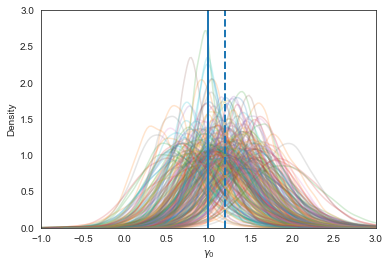
\includegraphics[width=\linewidth]{graphics/posterior_plot_gamma0_wrong}
    \caption{ N=200, J=10}
  \end{subfigure}
  \begin{subfigure}[b]{0.3\linewidth}
    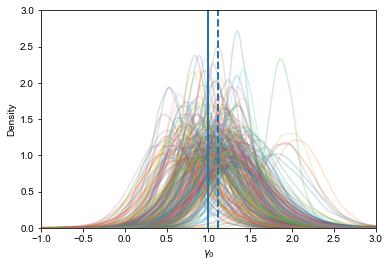
\includegraphics[width=\linewidth]{graphics/posterior_plot_gamma0_wrong_smallN}
    \caption{ N=100, J=10}
  \end{subfigure}
  \begin{subfigure}[b]{0.3\linewidth}
    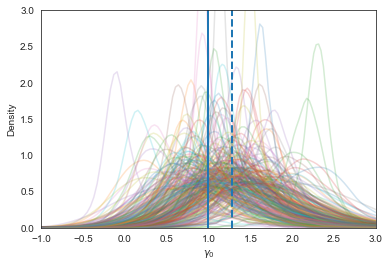
\includegraphics[width=\linewidth]{graphics/posterior_plot_gamma0_wrong_smallJ}
    \caption{N=200, J=5}
  \end{subfigure}
  \caption{Posterior densities of $\gamma_0$ with wrong prior, Blue line: True Value, Dotted line: Average Estimate}
  \label{fig:posterior_wrong_gamma0}
\end{figure}


\begin{figure}[h!]
  \centering
  \begin{subfigure}[b]{0.3\linewidth}
    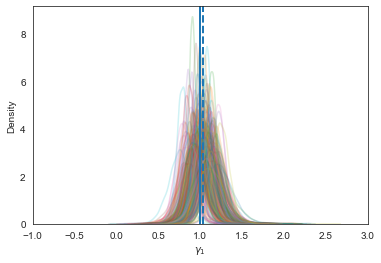
\includegraphics[width=\linewidth]{graphics/posterior_plot_gamma1_wrong}
    \caption{ N=200, J=10}
  \end{subfigure}
  \begin{subfigure}[b]{0.3\linewidth}
    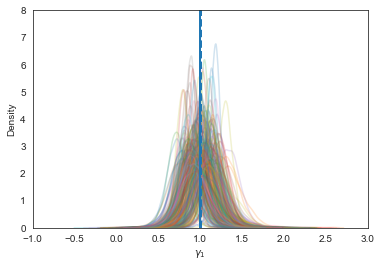
\includegraphics[width=\linewidth]{graphics/posterior_plot_gamma1_wrong_smallN}
    \caption{ N=100, J=10}
  \end{subfigure}
  \begin{subfigure}[b]{0.3\linewidth}
    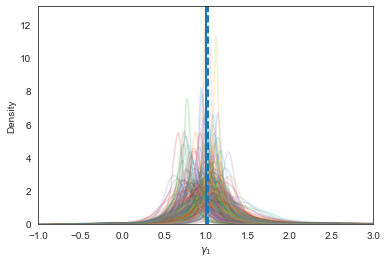
\includegraphics[width=\linewidth]{graphics/posterior_plot_gamma1_wrong_smallJ}
    \caption{N=200, J=5}
  \end{subfigure}
  \caption{Posterior densities of $\gamma_1$ with wrong prior, Blue line: True Value, Dotted line: Average Estimate}
  \label{fig:posterior_wrong_gamma1}
\end{figure}


%BIAS analysis
\begin{table}[!ht]
\begin{center}
\begin{tabular}{l  l  l  l  l  l  l  }
prior & \# classes & \#  students per class & $\gamma_0$ & $\gamma_1$\\
(def. in table)  & J  & N &  [1] &  [1] \\
\hline
%$\gamma_0=1, \gamma_1=1, \mu_x=\mu_u=5,\sigma_u=\sigma_x=0.3$\\
true & 8  &  200  &  1.002  &  0.9985 \\
true & 10  &  200  &  1.0089  &  0.9835 \\
weakwrong(just 80 runs) & 10  &  200  &  0.9033  &  1.5117\\
wrong & 10  &  200  &  0.865  &  1.7222\\
\end{tabular}
\end{center}
\caption{DGP1:Average posterior means of the \emph{random slope model} with different classsizes and number of schools. In square brackets: True parameter values.}
\label{tab:bias_first}
\end{table}

%BIAS analysis
\begin{table}[!ht]
\begin{center}
\begin{tabular}{l  l  l  l  l  l  l  }
prior & \# classes & \#  students per class & $\gamma_0$ & $\gamma_1$  & $\sigma_b$ & $\sigma_y$ \\
(def. in table)  & J  & N &  [1] &  [1]  & [1] & [1] \\
\hline
%$\gamma_0=1, \gamma_1=1, \mu_x=\mu_u=0,\sigma_u=\sigma_x=3$\\
true & 10  &  200  &  1.007  &  1.0355  &  1.1424  &  1.0001\\
wrong & 10  &  200  &  1.0376  &  1.1918  &  1.1587  &  1.0001\\
weakwrong & 10  &  200  &  1.0117  &  1.0622  &  1.1579  &  1.0001\\
weakslightlywrong & 10  &  200  &  1.0084  &  1.0448  &  1.1573  &  1.0001\\
uni &10  &  200  &  1.008  &  1.0415  &  1.1609  &  1.0001\\
\hline
true &10  &  100  &  0.9907  &  0.9921  &  1.161  &  1.0008\\
wrong & 10  &  100  &  1.009  &  1.1154  &  1.1752  &  1.0008\\
weakwrong & 10  &  100  &  0.9927  &  1.0082  &  1.1767  &  1.0007\\
weakslightlywrong & 10  &  100  &  0.9905  &  0.9954  &  1.176  &  1.0007\\
uni & 10  &  100  &  0.9906  &  0.9911  &  1.1791  &  1.0008\\
\hline
true & 5  &  200  &  0.9859  &  1.014  &  1.3556  &  1.0006\\
wrong & 5  &  200  &  1.0216  &  1.2784  &  1.4418  &  1.0006\\
weakwrong & 5  &  200  &  0.9885  &  1.0768  &  1.4886  &  1.0006\\
weakslightlywrong& 5  &  200  &  0.9858  &  1.0292  &  1.4832  &  1.0006\\
uni & 5  &  200  &  0.9851  &  1.0217  &  1.5577  &  1.0006\\
\end{tabular}
\end{center}
\caption{Average  posterior means of the \emph{random slope model}  with different classsizes and number of schools. In square brackets: True parameter values.}
\label{tab:bias_second}
\end{table}


% MEAN analysis
\begin{table}[!ht]
\begin{center}
\begin{tabular}{l l l l  l}
prior & \# classes & \#  students per class &  $\gamma_0$ & $ \gamma_1$ \\
\hline
%$\gamma_0=1, \gamma_1=1, \mu_x=\mu_u=5,\sigma_u=\sigma_x=0.3$
\hline
%$\gamma_0=1, \gamma_1=1, \mu_x=\mu_u=0,\sigma_u=\sigma_x=3$
true & 10  &  200  &  [0.52350012 1.48718419]  &  [0.84684044 1.15146533]\\
wrong &10  &  200  &  [0.69385994 1.63914985]  &  [0.89002761 1.17728129]\\
weakwrong & 10  &  200  &  [0.4942632 1.5721827]  &  [0.83996581 1.15165514]\\
weakslightlywrong & 10  &  200  &  [0.46322949 1.54766233]  &  [0.83877618 1.14408323]\\
uni & 10  &  200  &  [0.46317824 1.56124735]  &  [0.83470166 1.15248057]\\
\hline
true &10  &  100  &  [0.54092855 1.3524135 ]  &  [0.81665204 1.1720142 ]\\
wrong & 10  &  100  &  [0.6639 1.4909]  &  [0.8269 1.1853]\\
weakwrong & 10  &  100  &  [0.4913 1.4196]  &  [0.8143 1.1844]\\
weakslightlywrong & 10  &  100  &  [0.47016138 1.3994245 ]  &  [0.81024912 1.17970086]\\
uni & 10  &  100  &  [0.45852881 1.40629722]  &  [0.81510324 1.17769335]\\
\hline
true & 5  &  200  &  [0.44774977 1.57488554]  &  [0.7584738  1.17924577]\\
wrong & 5  &  200  &  [0.75601786 1.78479991]  &  [0.77873153 1.21025548]\\
weakwrong & 5  &  200  &  [0.32753143 1.73564282]  &  [0.74647839 1.19358118]\\
weakslightlywrong &5  &  200  &  [0.29528862 1.69647704]  &  [0.74279569 1.18609201]\\
uni & 5  &  200  &  [0.23926888 1.73950513]  &  [0.73225064 1.1940273 ]\\
\end{tabular}
\end{center}
\caption{ [0.05,0.95] percentiles of the (mean) estimates of the  \emph{random slope model}  with different classsizes and number of schools. }
\label{tab:means}
\end{table}

% quantiles: add \sigma_b and \sigma_y here!!!
\begin{table}[!ht]
\begin{center}
\begin{tabular}{l l l l  l}
prior & \# classes & \#  students per class &  $\gamma_0$ & $ \gamma_1$ \\
\hline
%First DGP & - & -& -& -& \\
%$\gamma_0=1, \gamma_1=1, \mu_x=\mu_u=5,\sigma_u=\sigma_x=0.3$
%true & 8 & 200 & [-0.6057, 2.6052] &[0.6494, 1.3539] \\
%true & 10  &  200  &  [-0.5925,2.5579]  &  [0.6642,1.3539]\\
%wrong&10  &  200  &  [0.1415,3.3019]  &  [0.5202,1.2112]\\
%weakwrong(just 80 runs) &  10  &  200  &  [-2.6723,5.7302]  &  [0.0334,1.7674]\\
\hline
%$\gamma_0=1, \gamma_1=1, \mu_x=\mu_u=0,\sigma_u=\sigma_x=3$
true & 10  &  200  &  [0.4427,1.627]  &  [0.8173,1.1965] \\ %0.9633 
wrong & 10  &  200  &  [0.6086,1.8279]  &  [0.8499,1.2383]\\ % 0.91
weakwrong & 10  &  200  &  [0.4134,1.7218]  &  [0.8163,1.209] \\  %  0.9367
weakslightlywrong & 10  &  200  &  [0.3929,1.6994]  &  [0.8125,1.2044]\\ % 0.9467
uni & 10  &  200  &  [0.3756,1.7065]  &  [0.8101,1.2059]\\ % 0.9467
\hline
true &10  &  100  &  [0.4275,1.5581]  &  [0.754,1.2283]\\
wrong&  10  &  100  &  [0.5581,1.7167]  &  [0.7727,1.255]\\
weakwrong & 10  &  100  &  [0.3912,1.6341]  &  [0.7482,1.2375]\\
weakslightlywrong &10  &  100  &  [0.3765,1.6175]  &  [0.7463,1.2345]\\
uni & 10  &  100  &  [0.3618,1.6206]  &  [0.7449,1.2368]\\
\hline
true & 5  &  200  &  [0.1868,1.8385]  &  [0.637,1.3362]\\
wrong & 5  &  200  &  [0.4655,2.242]  &  [0.6689,1.4232]\\
weakwrong & 5  &  200  &  [-0.0235,2.2405]  &  [0.5829,1.3996]\\
weaklightlywrong &5  &  200  &  [-0.0935,2.1598]  &  [0.5813,1.3925]\\
uni &5  &  200  &  [-0.2434,2.2897]  &  [0.5518,1.419]\\
\end{tabular}
\end{center}
\caption{ Average [0.05,0.95] percentiles of the \emph{random slope model}  with different classsizes and number of schools. }
\label{tab:quantiles}
\end{table}

% coverage ratio
\begin{table}[!ht]
\begin{center}
\begin{tabular}{l l l l  l}
prior & \# classes & \#  students per class &  $\gamma_0$ & $ \gamma_1$ \\
\hline
%$\gamma_0=1, \gamma_1=1, \mu_x=\mu_u=5,\sigma_u=\sigma_x=0.3$
\hline
%$\gamma_0=1, \gamma_1=1, \mu_x=\mu_u=0,\sigma_u=\sigma_x=3$
true & 10  &  200  &  0.9867  &  0.97\\
wrong & 10  &  200  &  0.97  &  0.98\\
weakwrong & 10  &  200  &  0.9767  &  0.9767\\
weakslightlywrong & 10  &  200  &  0.9833  &  0.9733\\
uni & 10  &  200  &  0.9833  &  0.9733\\
\hline
true &10  &  100  &  0.9767  &  0.9733\\
wrong & 10  &  100  &  0.9767  &  0.98\\
weakwrong & 10  &  100  &  0.97  &  0.9733 \\
weakslightlywrong &10  &  100  &  0.97  &  0.97\\
uni &10  &  100  &  0.9733  &  0.9767\\ 
\hline
true & 5  &  200  &  0.9833  &  0.9833\\
wrong & 5  &  200  &  0.9633  &  0.9833\\
weakwrong & 5  &  200  &  0.98  &  0.99\\
weakslightlywrong &5  &  200  &  0.9767  &  0.99\\
uni &5  &  200  &  0.98  &  0.9833\\
\end{tabular}
\end{center}
\caption{[0.05,0.95] coverage \emph{random slope model}  with different classsizes and number of schools. }
\label{tab:coverage}
\end{table}


% MEDIAN
\begin{table}[!ht]
\begin{center}
\begin{tabular}{l l l l  l}
prior & \# classes & \#  students per class &  $\gamma_0$ & $ \gamma_1$ \\
\hline
wrong &10  &  100  &  [0.6415 1.4825]  &  [0.8219 1.184 ]\\
weakwrong & 10  &  100  &  [0.4894 1.4232]  &  [0.8105 1.1806]\\
\hline
\end{tabular}
\end{center}
\caption{ [0.05,0.95] percentiles of the (median) estimates of the  \emph{random slope model}  with different classsizes and number of schools. }
\label{tab:median}
\end{table}